%%%%%%%%%%%%%%%%%%%%%%%%%%% asme2ej.tex %%%%%%%%%%%%%%%%%%%%%%%%%%%%%%%
% Template for producing ASME-format journal articles using LaTeX    %
% Written by   Harry H. Cheng, Professor and Director                %
%              Integration Engineering Laboratory                    %
%              Department of Mechanical and Aeronautical Engineering %
%              University of California                              %
%              Davis, CA 95616                                       %
%              Tel: (530) 752-5020 (office)                          %
%                   (530) 752-1028 (lab)                             %
%              Fax: (530) 752-4158                                   %
%              Email: hhcheng@ucdavis.edu                            %
%              WWW:   http://iel.ucdavis.edu/people/cheng.html       %
%              May 7, 1994                                           %
% Modified: February 16, 2001 by Harry H. Cheng                      %
% Modified: January  01, 2003 by Geoffrey R. Shiflett                %
% Use at your own risk, send complaints to /dev/null                 %
%%%%%%%%%%%%%%%%%%%%%%%%%%%%%%%%%%%%%%%%%%%%%%%%%%%%%%%%%%%%%%%%%%%%%%

%%% use twocolumn and 10pt options with the asme2ej format
\documentclass[twocolumn,10pt]{asme2ej}
\usepackage{graphicx}
\usepackage{epsfig} %% for loading postscript figures

%% The class has several options
%  onecolumn/twocolumn - format for one or two columns per page
%  10pt/11pt/12pt - use 10, 11, or 12 point font
%  oneside/twoside - format for oneside/twosided printing
%  final/draft - format for final/draft copy
%  cleanfoot - take out copyright info in footer leave page number
%  cleanhead - take out the conference banner on the title page
%  titlepage/notitlepage - put in titlepage or leave out titlepage
%  
%% The default is oneside, onecolumn, 10pt, final


\title{The Rise of the Airbnb Empire}

%%% first author
\author{Christine Chae Hwang
    \affiliation{
	Senior, Statistics Department
	Harvard University\\
	Class of 2017\\
    Email: chaehwang@college.harvard.edu
    }	
}
\author{Michael Parzen
    \affiliation{
    	Advisor
	Statistics Department
	Harvard University\\
    }	
}


\begin{document}

\maketitle    

%%%%%%%%%%%%%%%%%%%%%%%%%%%%%%%%%%%%%%%%%%%%%%%%%%%%%%%%%%%%%%%%%%%%%%
\begin{abstract}
{\it 
%%% 
This paper delves into the driving factors of the growing prices of Airbnb rentals in Los Angeles. We not only want to provide a tool for the home owners that can help them decide a competitive price for their listing given the characteristics of their home, but also gain a deeper understanding of what features are the most important to consumers that drive the prices. In this model, we explore a classification method that can project a bucket or a price range to project a general price. The models we consider are Logistic Regression, Linear Regression, and Random Forest Classifier.
}
\end{abstract}

\section{Introduction}
\subsection{Background}
Housing in Los Angeles has risen tremendously over the past couple of years. As the job market is increasing and the tourism industry grows, hotel prices and rent is rising tremendously. Interns in search of sublets often cannot afford these high prices and are looking for cheaper alternatives for housing in LA. As the housing market grows more and more expensive, Airbnb has acquired a lot of popularity for short term stays ranging anywhere from a weekend trip to a three month internship sublet. Understanding what drives these factors and building a model that can accurately project the price of a listing given its properties will have positive consequences for both the consumer and the provider
\subsection{Motivation}
As more and more home owners want to partake in this market, it becomes ambiguous what a competitive and appropriate price for their listing would be. With this model, a home owner can simply input the characteristics of their home and understand what a competitive price would be, helping them make the decision if they should enter the Airbnb market or not and project their income. In addition, it helps us understand what consumers are looking for when they book an Airbnb. While many listing owners may think that the number of beds available and bathrooms are the driving factors for price, those in search of temporary housing may actually be willing to pay more only based on the location and disregard the size of the listing. By conducting this analysis, we are better able to parse out the consumer's needs and inform the listing owners what the valuable features of their homes may be. Therefore, this research benefits both the consumers and providers by increasing the supply of desirable listings and project competitive prices for new listings.
%%%%%%%%%%%%%%%%%%%%%%%%%%%%%%%%%%%%%%%%%%%%%%%%%%%%%%%%%%%%%%%%%%%%%%
\section{Data Explorations}
\subsection{Initial Features}
In the dataset provided by http://insideairbnb.com/get-the-data.html, there were a myriad of features that were worth exploring for this project.  Because of the high dimensionality, I want to be intentional in the variables I include in my study. I wanted to include variables that indicate the size of the listing: number of bedrooms, bathrooms, beds, square footage. I also wanted to include variables that indicate customer satisfaction: Number of reviews, average review rating, and sentiment analysis of the comments. I also wanted to include information about the location: zipcode, distance to nearest transportation, nearby attraction sites. Lastly, I want to include information about the host and his or her personality: encaptured by the listing description, host identity verified, name of listing, etc. 

\subsection{Transformation}
From basic data exploration, some of the features were heavily skewed. As expected, our target variable, price was very heavily skewed to the right.  add this in appendix and do the figure blah stuff.

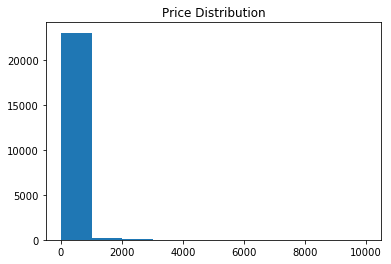
\includegraphics[scale=.5]{price.png}

Because some models, such as linear regression assume a normally distributed target variable, I took the log of the price so that such assumptions were not violated in the model.

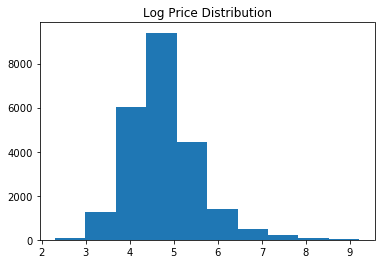
\includegraphics[scale=.5]{log_price.png}
\section{Feature Extraction}
Using the features provided, I wanted to generate some of my own features that I thought would be advantageous in predictive power.
\subsection{Buzzwords First-Level Model}
The qualitative data points are sometimes difficult to use in model building, but carry very important informational value that could that high predictive power. In the summary and description that the host uploads, there could be certain buzzwords such as "beach" or "view" that drive up the prices drastically. To account for this, I vectorized each of the words in the blurbs of textual data and regressed this to the price using a Random Forest Regressor. I then selected the top 10 words that had the highest positive correlation with price and deemed these "buzzwords" to high prices.
\begin{center}
\begin{tabular}{ |c|c|c| } 
\hline
  {\bf{Ranking}} &{\bf{Name}} & {\bf{ Description}} \\ 

 \hline
 1 & traverse & pasadena \\ 
 \hline
 2 & elite & designed \\ 
 \hline
 3 & estate & spanish \\ 
 \hline
 4 & beach & beverly \\ 
 \hline
  5 & cod & claremont \\ 
 \hline
  6 & unbelievable & secured \\ 
 \hline
  7 & villa & exclusive \\ 
 \hline
  8 & paradise & 3ba \\ 
 \hline
  9 & 6bd & distances \\ 
 \hline
 10 & malibu & crescenta \\ 
 \hline
\end{tabular}
\end{center}
It seems from the description that the highest priced Airbnbs are safe and exclusive. Desired locations include Beverly Hills, Claremont and Pasadena. Buzzwords to use when you are naming your listing is "elite" and "paradise". Consumers seem to also pay a premium for beach houses which is likely correlated with malibu. 
\begin{center}
\begin{tabular}{ |c|c|c| } 
\hline
  {\bf{Ranking}} &{\bf{House Rules}} & {\bf{ Transit}} \\ 

 \hline
 1 & pets & 10miles \\ 
 \hline
 2 & refrain & 2 mins \\ 
 \hline
 3 & politely & 4 mins \\ 
 \hline
 4 & wild & parking \\ 
 \hline
  5 & balcony & freeway \\ 
  \hline
\end{tabular}
\end{center}

From the house rules, the words seem to suggest that Airbnbs that are in close proximity to a major attraction and offer parking are desirable. Likely because LA is mainly commuted using cars, location is a huge plus for LA Airbnbs. House rules did not seem to show a specific insight in terms of premium.

\subsubsection{Discussion}
From the analysis of the Buzzwords, it seems like location is a much stronger driver factor of a higher price than the size of the listing. Altho words such as 3 bathroom did show up, words that described the location and distance from major attractions seemed to land in the top 10 buzzwords much more often. One caveat and drawback to this methodology of identifying buzzwords is that there could be outliers that influence the weight of a single word. In addition, the magnitude of the English vocabulary is quite large and leads to a sparse data set. However, to get a high level idea of buzzwords, this method does its job.
\subsection{Qualitative Transformation}
While understanding the buzzwords is useful for the listings owner when they put out a new home for rent, it can also be a powerful predictive variable. In order to condense the qualitative information to a single number to feed into a single variable, I extracted the top 50 buzzwords into a list and created a weighted score by counting how many times a given description has a buzzwords and multiplying it by its "rank" which is defined by the order of variable importance.
\subsection{Indicator Variables}
In addition the presence of buzzwords, the absence of words at all also plays a factor in the price of the listing. Therefore, for all the listings that do not indicate any description or words on the transit could be a negative influence on the price, which I want to consider as well. Therefore, I include indicator variables that signal missing data. For the remaining missing values, I filled it with 0.
\section{Models}
After data processing and formatting the features such that the input of the data into the algorithm can be represented by a numpy array, I ran 4 different classification models and tuned corresponding parameters to find the best performing model. I categorized the target variable to land in 3 different buckets- high, medium, low. Low price corresponds to , medium corresponds to , and high corresponds to. 
\subsection{Classification}
The models we took into consideration are Random Forest Classifier, SVM and Logistic Regression. We tuned the num estimators for the random forest, the C parameter for SVM and the C parameter for logistic regression. Using cross validation, we selected the parameters that resulted in the highest overall accuracy. 
\begin{center}
\begin{tabular}{ |c|c|c| } 
\hline
  {\bf{Model}} & {\bf{Accuracy}}  \\ 
 \hline
 Random Forest &   .749\\ 
 \hline
 SVM &   .505\\ 
 \hline
 Logistic Regression & .7307  \\ 
 \hline
\end{tabular}
\end{center}

We can see from the table above that the Random Forest Classifier performed the best out of all the models with an accuracy of .749. The Random Forest is often a very robust model that is less prone to overfitting than other models because they have a random ensemble of trees that account for the variance.
\section{Feature Importances}
The important features that had the most predictive power were bedrooms and whether it was an entire home rental.
\begin{center}
\begin{tabular}{ |c|c|c| } 
\hline
  {\bf{Variable}} & {\bf{Importance}}  \\ 
 \hline
 bedrooms &   .065\\ 
 \hline
 Entire Home/apt &   .065\\ 
 \hline
accommodates & .064  \\ 
 \hline
 private room & .048  \\ 
 \hline
 bathrooms & .045  \\ 
 \hline
 reviews per month & .042  \\ 
 \hline
  beds & .042  \\ 
 \hline
 house-quant & .032  \\ 
 \hline
 transit-quant & .029  \\ 
 \hline
\end{tabular}
\end{center} 
We can see from the feature importances that the top driving predictors still related to the size and the number of people this would accommodate. It seems that consumers are willing to pay high premiums for more bedrooms and bathrooms. In addition, it shows that there is a higher premium to rent an entire home/apt than there is to rent a private room, even if all other conditions are equivalent. Consumers also care about the quality of the listing as shown by the reviews per month, and that higher quality listings are more likely to charge higher rates. As we had predicted, though it did not have higher influence than the size of the room, the qualitative features listed in the house rules and transit description box had an impact on the price. If you recall, the house-quant and transit-quant refer to the number of buzzwords these descriptions have. Therefore, it shows that location does play a significant factor in influencing the price.
\section{Discussion}
Throughout this research and experiment, we have gained much insight regarding what consumers desire and how suppliers can package their listing that is most appealing to their audience. From our buzzword analysis, we saw that the listings should try their best to advertise the location of their house through the description and transit. Marketing how close their homes are to main attraction sites and public transportation proves to be lucrative. From the modeling, we see that the quantitative aspect of the house sells themselves. Consumers know where to find this information and it doesn't need to be directly addressed in the descriptions. In addition, consumers seem to prefer private houses that are active and spacious. 

\begin{acknowledgment}
I would like to thank Mike Parzen for allowing me to pursue this research project throughout the semester. I would also like to thank Airbnb for allowing me to utilize their dataset to reach these conclusions. Further code can be found the github link below.
\end{acknowledgment}

%%%%%%%%%%%%%%%%%%%%%%%%%%%%%%%%%%%%%%%%%%%%%%%%%%%%%%%%%%%%%%%%%%%%%%
% The bibliography is stored in an external database file
% in the BibTeX format (file_name.bib).  The bibliography is
% created by the following command and it will appear in this
% position in the document. You may, of course, create your
% own bibliography by using thebibliography environment as in
%
% \begin{thebibliography}{12}
% ...
% \bibitem{itemreference} D. E. Knudsen.
% {\em 1966 World Bnus Almanac.}
% {Permafrost Press, Novosibirsk.}
% ...
% \end{thebibliography}

% Here's where you specify the bibliography style file.
% The full file name for the bibliography style file 
% used for an ASME paper is asmems4.bst.
\bibliographystyle{asmems4}

% Here's where you specify the bibliography database file.
% The full file name of the bibliography database for this
% article is asme2e.bib. The name for your database is up
% to you.
\bibliography{asme2e}

%%%%%%%%%%%%%%%%%%%%%%%%%%%%%%%%%%%%%%%%%%%%%%%%%%%%%%%%%%%%%%%%%%%%%%

\end{document}
